%%%%%%%%%%%%%%%%%%%%%%%%%%%%%%%%%%%%%%%%%%%%%%%%%%%%%%%%%%%%%%%%%%%%%%%%%%%%%%%%%%%%%%%%%%%%%%%%%%%%%%%
\section{How the Tea Party Votes}
\label{sec:c6_teaparty}
%%%%%%%%%%%%%%%%%%%%%%%%%%%%%%%%%%%%%%%%%%%%%%%%%%%%%%%%%%%%%%%%%%%%%%%%%%%%%%%%%%%%%%%%%%%%%%%%%%%%%%%

In this section, we examine legislators' ideal points.  We first
expose Tea Party-specific ideal points by examining one-dimensional
ideal points and then move on to the issue-specific ideal points that
\name{} enables.

\ignore{
\subsection{Data Collection}
\label{subsec:c6_data}

What makes a Tea Partier?  To address that question, we use
\textit{key votes} identified by \fw{} as the most important votes on
issues of economic freedom.  Led by former House Majority Leader Dick
Armey (\abr{r-tx}), \fw{} is a conservative non-profit organization
that promotes ``Lower Taxes, Less Government, More
Freedom''.\footnote{\url{http://congress.freedomworks.org/}}
\newcite{Karpowitz:PS11:teaparty} report that \fw{} endorsements were
more effective than other Tea Party organizations at getting out votes
for Republican candidates in the 2010 midterms.

For the 112\textsuperscript{th} Congress, \fw{} selected 60 key votes,
40 in 2011 and 20 in 2012.  We are interested in ideal points with
respect to the Tea Party movement, i.e., on the anti-pro Tea Party
dimension: whether a legislator agrees with \fw{} on a bill. More
specifically, we assign $v \subtwo ab$ to be 1 if legislator $a$
agrees with \fw{} on bill $b$, and 0 otherwise. In total, we have 240
Republicans, 60 who self-identify with the Tea Party Caucus, and
13,856 votes.
}

\subsection{One-dimensional Ideal Points}
\label{subsec:c6_onedim_idealpoint}

First, as a baseline, we estimate the one-dimensional ideal points of
the legislators in our dataset.\footnote{We use gradient ascent to optimize the likelihood of votes whose probabilities are defined in Equation~\ref{eqn:c6_onedim}. We also put a Gaussian prior $\mathcal{N}(0,\sigma)$ on $u_a$, $x_b$, and $y_b$.}
Figure~\ref{fig:c6_onedim_112} shows the box plots of estimated Tea
Party ideal points for both members and
non-members.\footnote{Estimated ideal point signs might be flipped, as
  $u_a x_b = (-u_a)(-x_b)$, which makes no difference in
  Equation~\ref{eqn:c6_onedim}. To ensure that higher ideal points are
  ``pro-Tea Party'', we first sort the legislators according to the
  fraction of votes for which they agree with \fw{} and initialize the
  ideal points of the top and bottom five legislators with +3$\sigma$
  and -3$\sigma$, where $\sigma$ is the variance of $u_a$'s Gaussian
  prior.}  The Tea Party ideal points correlate with \dwnom{} ($\rho= 0.91$), and
the median ideal point of Tea Party Caucus members is higher than
non-members. This confirms that Tea Partiers are more conservative
than other
Republicans~\cite{Williamson:PP11,Karpowitz:PS11:teaparty,GervaisPSP12:tealeaves,Gervais:APSA14}.

% We put a Gaussian prior
% $\mathcal{N}(0, \sigma)$ over $u_a$, $x_b$ and $y_b$ and use gradient ascent to optimize the
% following log likelihood
% \begin{eqnarray}
% \small
% \mathcal{L}(\bm u, \bm x, \bm y)
%   &=& \sum_{a=1}^A \sum_{b=1}^B v \subtwo ab \log p(v \subtwo an = 1) + (1- v \subtwo ab)  \log p(v \subtwo ab = 0) \nonumber \\
%   &-& \frac{1}{2\sigma} \left(\sum_{a=1}^A u_a^2 + \sum_{b=1}^B x_b^2 + \sum_{b=1}^B y_b^2\right)
% \end{eqnarray}

\begin{figure}[t]
    \centering
  \includegraphics[width=.9\linewidth]{\autofig{onedim_ip_112}}
  \caption{Box plots of the one-dimensional Tea Party ideal
    points, estimated as a baseline in Section~\ref{subsec:c6_onedim_idealpoint}, for members and non-members of the Tea Party Caucus among
    Republican Representatives in the 112\textsuperscript{th} \us{}
    House.  The median of members' ideal points is significantly
    higher than that of non-members'.}
  \label{fig:c6_onedim_112}
\end{figure}

% \begin{figure}[t]
%     \centering
%     \begin{subfigure}[b]{0.49\linewidth}
%             \includegraphics[width=\textwidth]{2015_teaparty/auto_fig/bottom_onedim_ip}
%             \caption{}
%             \label{fig:c6_bottom_onedim}
%     \end{subfigure}%
%     \begin{subfigure}[b]{0.49\linewidth}
%             \includegraphics[width=\textwidth]{2015_teaparty/auto_fig/top_onedim_ip}
%             \caption{}
%             \label{fig:c6_top_onedim}
%     \end{subfigure}%
%     \caption{Republican legislators with the (a) lowest and (b) highest estimated one-dimensional ideal points.}
%     \label{fig:c6_top_bottom_onedim}
% \end{figure}

Divergences involving these ideal points help demonstrate the face
validity of our approach. For example, the model gives Jeff Flake (\abr{r-az}) the second highest ideal point; he only disagrees with Freedom Work’s position on one of 60 Freedom Works’ key votes, but he is not a member of the Tea Party Caucus. Another example is Justin Amash (\abr{r-mi}), who founded and is the Chairman of the Liberty Caucus. Its members are conservative and libertarian Republicans, and Amash has agreed with \fw{} on every single key vote selected by \fw{} since 2011.

Conversely, some self-identified Tea Partiers often disagree with \fw{} and thus have
relatively low ideal points. For example, Rodney Alexander (\abr{r-la}) only agrees
with \fw{} 48\% of the time, and was a Democrat before 2004. Alexander and
Ander Crenshaw (\abr{r-fl}, 50\% agreement) are categorized as ``Green
Tea'' by~\newcite{Gervais:APSA14}, i.e. Republican legislators who are
``associated with the Tea Party on their own initiative'' but lack
support from Tea Party organizations.

\subsection{Multi-dimensional Ideal Points}
\label{subsec:c6_multdim_idealpoint}

\begin{figure*}[t]
\centering
  %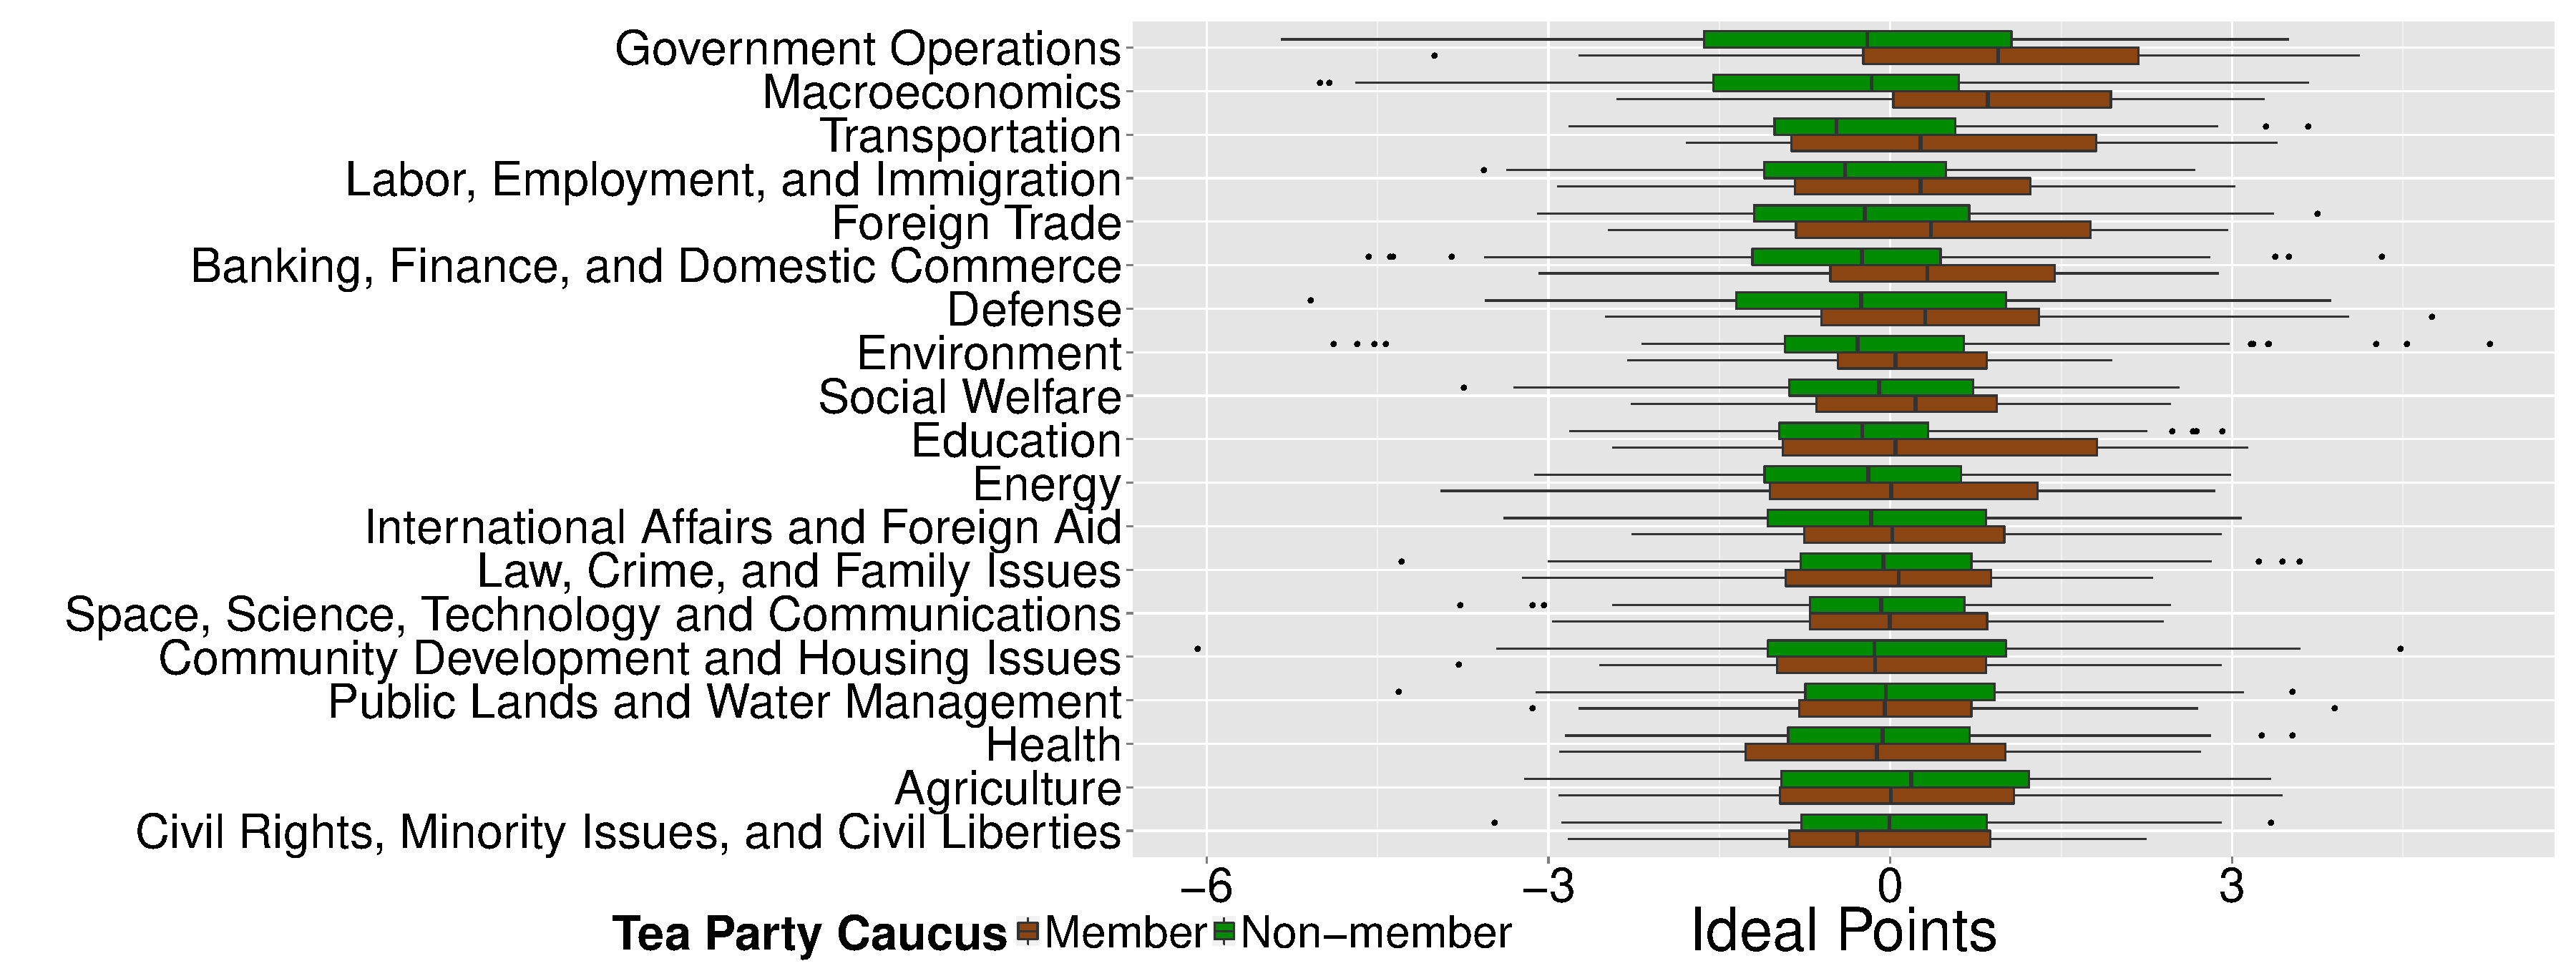
\includegraphics[width=.95\linewidth]{2015_teaparty/auto_fig/multdim_ip_112}
  \includegraphics[width=.78\linewidth]{\figfile{multdim_ip_112}}
  \caption{Box plots of ideal points dimensions, each corresponding
    to a major topic in the Policy Agendas Topics Codebook estimated by our model.  On
    most issues the ideal point distributions over the two Republican groups
    (member vs. non-member of the Tea Party Caucus) overlap. The
    most polarized issues are \underline{Government Operations} and \underline{Macroeconomics},
    which align well with the agenda of the Tea Party movement supporting small
    government and lower taxes.}
  \label{fig:c6_multdim_112}
\end{figure*}

While it is interesting to compare holistic measures of Tea Partiness,
it doesn't reveal \emph{how} legislators conform or deviate from what
defines a mainstream Tea Partier.  In this section, \name{} reveals
how \emph{issue-specific} ideal points of the two groups of Republican
representatives differ.

Figure~\ref{fig:c6_multdim_112} shows estimated ideal points
for each policy agenda issue, sorted by the difference between the median of the
two groups' ideal points. On most issues, the ideal point distributions of the
two Republican groups are nigh identical.

On several issues, though, the ideal point distributions of the two groups of
legislators diverge.
%  To understand why these issues polarize, we
% look at key votes. Recall that in our model, each bill $b$ has a distribution
% $\vartheta_b$ over $K$ issues, capturing what the bill is about. For each key
% vote $b$, we choose the issue with the highest probability $\vartheta \subtwo
% bk$ and use it to label. Although using a single issue for each key vote
% conflicts with our model's admixture assumption in which each document is a
% mixture of topics, it provides a good estimation of what the key vote is
% primarily about and helps reduce the complexity of our analysis.
In the remainder of this section, we consider the
\underline{Government Operation}, \underline{Macroeconomics}, and
\underline{Transportation} topics, and look at why \name{} estimates these issues as
the most polarized.

\paragraph{Government operations}

Tea Partiers differ from their Republican colleagues on reducing
government spending on the Economic Development Administration, the
Energy Efficiency and Renewable Energy Program and Fossil Fuel
Research and Development. More specifically, for example, on the key
vote \textit{to eliminate the Energy Efficiency and Renewable Energy
  Program}, nearly 80\% (41 out of 53) of Tea Partiers vote ``Yea''
(with \fw{}) but only 43\% of non-Tea Partiers agree.

% \begin{table}
% \centering \small
% \begin{tabular}{|c|m{.30\textwidth}|c|ccc|ccc|c|}
%   \hline
%     \multirow{2}{*}{ID} & \multirow{2}{*}{Key vote title} & \multirow{2}{*}{FW}
%         & \multicolumn{3}{c|}{\# Agrees}
%         & \multicolumn{3}{c|}{\# Disagrees}
%         & \multirow{2}{*}{$\vartheta \subtwo bk$} \\
%         & & & All & \tp{TP} & \ntp{NTP} & All & \tp{TP} & \ntp{NTP} & \\ \hline
%     2012-221 & To cut Commerce, Science, \& Justice appropriations by 1\%
%         & Y & 156 & \tp{48} & \ntp{108} & 77 & \tp{10} & \ntp{67} & .47 \\ \hline
%     \textbf{2012-207} & \textbf{To eliminate the Economic Development Administration}
%         & Y & 128 & \tp{45} & \ntp{83} & 104 & \tp{14} & \ntp{90} & .46 \\ \hline
%     \textbf{2012-222} & \textbf{To cut \$2.7 billion from selected portions of CJS appropriations}
%         & Y & 105 & \tp{35} & \ntp{70} & 128 & \tp{23} & \ntp{105} & .46 \\ \hline
%     \textbf{2012-311} & \textbf{To eliminate the Energy Efficiency and Renewable Energy Program}
%         & Y & 114 & \tp{41} & \ntp{73} & 106 & \tp{12} & \ntp{94} & .39 \\ \hline
%     \textbf{2012-336} & \textbf{To cut \$3.1 billion from Energy and Water appropriations}
%         & Y & 125 & \tp{43} & \ntp{82} & 110 & \tp{15} & \ntp{95} & .36 \\ \hline
%     \textbf{2012-317} & \textbf{To defund the Fossil Fuel Research and Development programs}
%         & Y & 102 & \tp{39} & \ntp{63} & 123 & \tp{19} & \ntp{104} & .35 \\ \hline
%     2012-513 & To require a full audit of the Federal Reserve System and the Federal reserve banks
%         & Y & 237 & \tp{60} & \ntp{177} & 1 & \tp{0} & \ntp{1} & .35 \\ \hline
%     \textbf{2011-538} & \textbf{To cut spending 9.93\% (\$3.04 billion) from Energy \& Water Appropriations Act of 2012}
%         & Y & 95 & \tp{34} & \ntp{61} & 135 & \tp{22} & \ntp{113} & .32 \\ \hline
%     2012-450 & Making appropriations for the Departments of Transportation, and Housing and Urban Development
%         & N & 54 & \tp{22} & \ntp{32} & 182 & \tp{36} & \ntp{146} & .31 \\ \hline
%     \textbf{2011-434} & \textbf{To cut \$900 million in waste and apply to a spending reduction account}
%         & Y & 108 & \tp{38} & \ntp{70} & 128 & \tp{22} & \ntp{106} & .30 \\ \hline
%     \textbf{2011-424} & \textbf{To cut \$700 million dollars in waste to pay off the debt}
%         & Y & 82 & \tp{32} & \ntp{50} & 151 & \tp{28} & \ntp{123} & .30 \\ \hline
% \end{tabular}
% \caption{Key votes having ``Government operations'' as the most probable issue, estimated by our
% model. The last column shows the estimated probability $\vartheta \subtwo bk$. Each key vote is
% shown with a short description, the preferred voting position of \fw{} (Y for Yea, N for Nay), the
% number of Republicans whose votes agree and disagree with \fw{} (`All' denotes all voting
% Republican legislators, `\tp{TP}' denotes Tea Party Caucus members, and `\ntp{NTP}' denotes non-Tea
% Party Caucus members). Bolded key votes are the ones on which the majority of the two groups vote
% differently.} \label{tab:c6_gov_opt}
% \end{table}

\paragraph{Macroeconomics}

% \begin{table}
% \centering \small
% \begin{tabular}{|c|m{.3\textwidth}|c|ccc|ccc|c|}
%   \hline
%     \multirow{2}{*}{ID} & \multirow{2}{*}{Key vote title} & \multirow{2}{*}{FW}
%         & \multicolumn{3}{c|}{\# Agrees}
%         & \multicolumn{3}{c|}{\# Disagrees}
%         & \multirow{2}{*}{Est} \\
%         & & & All & \tp{TP} & \ntp{NTP} & All & \tp{TP} & \ntp{NTP} & \\ \hline
%     \textbf{2011-275} & \textbf{To replace the Paul Ryan budget with the RSC's budget}
%         & Y & 118 & \tp{45} & \ntp{73} & 119 & \tp{15} & \ntp{104} & 0.85 \\ \hline
%     2011-277 & Congressman Paul Ryan's Budget for Fiscal Year 2012
%         & Y & 234 & \tp{58} & \ntp{176} & 3 & \tp{2} & \ntp{1} & 0.84 \\ \hline
%     \textbf{2012-149} & \textbf{Substitute amendment containing the Republican Study Committee budget for FY 2013}
%         & Y & 135 & \tp{50} & \ntp{85} & 104 & \tp{10} & \ntp{94} & 0.78 \\ \hline
%     2011-690 & The Budget Control Act of 2011
%         & N & 65 & \tp{27} & \ntp{38} & 173 & \tp{33} & \ntp{140} & 0.74 \\ \hline
%     2011-162 & Small Business Paperwork Mandate Elimination Act of 2011
%         & Y & 236 & \tp{60} & \ntp{176} & 0 & \tp{0} & \ntp{0} & 0.71 \\ \hline
%     2011-606 & Cut, Cap, and Balance Act
%         & Y & 229 & \tp{58} & \ntp{171} & 8 & \tp{2} & \ntp{6} & 0.69 \\ \hline
%     2012-32 & To amend the Balanced Budget and Emergency Deficit Control Act of 1985 to reform the budget baseline
%         & Y & 231 & \tp{57} & \ntp{174} & 0 & \tp{0} & \ntp{0} & 0.64 \\ \hline
%     2012-659 & On Concurring with the Senate Amendments: H.R. 8 - Taxpayer Relief Act of 2012
%         & N & 150 & \tp{50} & \ntp{100} & 84 & \tp{9} & \ntp{75} & 0.57 \\ \hline
%     2011-14 & Repealing the Job-Killing Health Care Law Act
%         & Y & 238 & \tp{60} & \ntp{178} & 0 & \tp{0} & \ntp{0} & 0.51 \\ \hline
%     2011-901 & Making major executive regulations subject to Congressional vote (REINS Act)
%         & Y & 236 & \tp{59} & \ntp{177} & 0 & \tp{0} & \ntp{0} & 0.49 \\ \hline
% \end{tabular}
% \caption{Key votes having ``Macroeconomics'' as the most probable issue, estimated by our model.
% The last column shows the estimated probability $\vartheta \subtwo bk$. Each key vote is shown with
% a short description, the preferred voting position of \fw{} (Y for Yea, N for Nay), the number of
% Republicans whose votes agree and disagree with \fw{} (`All' denotes all voting Republican
% legislators, `\tp{TP}' denotes Tea Party Caucus members, and `\ntp{NTP}' denotes non-Tea Party
% Caucus members). Bolded key votes are the ones on which the majority of the two groups vote
% differently.} \label{tab:c6_macroeconomics}
% \end{table}

Our model estimates \underline{Macroeconomics} policies as being the second most polarizing topic for House Republicans, which is consistent with the emphasis that the Tea Party places on issues like a balanced budget and reduced federal spending. Indeed, we see that Tea Party Republicans have distinct preferences on these types of issues as compared to more mainstream Republican legislators. An illustration of this polarization can be seen in the intra-party fight over the budget. Roll call vote 275 in 2011 and roll call vote 149 in 2012 both would have replaced Paul Ryan's budget (the ``establishment'' Republican budget) with the Republican Study Committee's (\abr{rsc}) ``Back to Basics'' budget that would cut spending more aggressively and balance the budget in a decade. In 2011, non-Tea Party Republicans were evenly split in their budget preferences, but three quarters of the Tea Party Caucus supported it, which illustrates the difference between the two factions of the Republican party. Similarly, in 2012, more than 80\% of Tea Partiers voted for the the RSC budget, but fewer than half of non-Tea Party Republicans did. Other polarizing votes in the Macroeconomics topic include votes to raise the debt ceiling and to avert the ``fiscal cliff''. In these cases, support for these votes was 25 percentage points higher among Tea Partiers than non-Tea Party Republicans, which again illustrates their distinct policy preferences.

\ignore{
\url{http://congress.freedomworks.org/bills/house-concurrent-resolution-hcres-or-hconres-34?keyvote=9470&tab=roll-call}
\url{http://congress.freedomworks.org/bills/house-concurrent-resolution-hcres-or-hconres-112?keyvote=10360&tab=roll-call}
}

\ignore{
Among \underline{Macroeconomics} votes, there are two key votes where the two
groups vote differently.  These are key vote 2011--275 (\textit{To
  replace the Paul Ryan budget with the RSC's budget}) and key vote
2012--149 (\textit{Substitute amendment containing the Republican
  Study Committee budget for FY 2013}). Both replace Paul Ryan's
budget with the Republican Study Committee's (\abr{rsc})
 ``Back to Basics'' to cut government spending more
aggressively and balance the budget in a decade. In 2011, this split
the Republicans evenly, but three quarters of the Tea Party Caucus
voted for it. In 2012, even more Tea Partiers voted for it,
while there were still more than half of non-Tea Party Caucus members
voting against it.  Other polarizing votes were to raise the debt
ceiling and avert the ``fiscal cliff''. {\bf PSR: Kris, please fix
  this paragraph; I can't make sense of it. Also, what happened to
  Finance? Too close to Macroeconomics? Do we need to explain why we
  skip it?}
  }

\paragraph{Transportation}

% \begin{table}
% \centering \small
% \begin{tabular}{|c|m{.3\textwidth}|c|ccc|ccc|c|}
%   \hline
%     \multirow{2}{*}{ID} & \multirow{2}{*}{Key vote title} & \multirow{2}{*}{FW}
%         & \multicolumn{3}{c|}{\# Agrees}
%         & \multicolumn{3}{c|}{\# Disagrees}
%         & \multirow{2}{*}{Est} \\
%         & & & All & \tp{TP} & \ntp{NTP} & All & \tp{TP} & \ntp{NTP} & \\ \hline
%     \textbf{2012-378} & \textbf{To require that transportation spending be capped}
%         & Y & 82 & \tp{32} & \ntp{50} & 145 & \tp{23} & \ntp{122} & 0.58 \\ \hline
%     2012-451 & To provide an extension of Federal-aid highway ... transit, and other programs
%         & N & 51 & \tp{20} & \ntp{31} & 186 & \tp{38} & \ntp{148} & 0.57 \\ \hline
% \end{tabular}
% \caption{Key votes having ``Transportation'' as the most probable issue, estimated by our model.
% The last column shows the estimated probability $\vartheta \subtwo bk$. Each key vote is shown with
% a short description, the preferred voting position of \fw{} (Y for Yea, N for Nay), the number of
% Republicans whose votes agree and disagree with \fw{} (`All' denotes all voting Republican
% legislators, `\tp{TP}' denotes Tea Party Caucus members, and `\ntp{NTP}' denotes non-Tea Party
% Caucus members). Bolded key votes are the ones on which the majority of the two groups vote
% differently. Both of these votes focus on the federal spending } \label{tab:c6_transportation}
% \end{table}

\underline{Transportation} is the third most polarized issue estimated by our model, with two key votes focusing on federal spending on transportation that illustrate some polarization, but also some shared preferences among Republicans. Consistent with the Tea Party's emphasis on reducing government spending, Tea Party Republicans voted differently from their non-Tea Party colleagues on these issues. The first key vote, roll call vote 378 in 2012, caps highway spending at the amount taken in by the gas tax. More than half of Tea Party Caucus members (32 out of 55) voted in favor, while non-members voted against it by a greater than 2:1 margin (122 of 172). Conversely, the second key vote (roll call vote 451 in 2012) authorizes federal highway spending at a level that far exceeds its revenue from the gas tax, which was opposed by \fw{}.  This measure was broadly popular with Republicans regardless of Tea Party affiliation and a majority of both Tea Partiers and non-Tea Partiers opposed it.

\ignore{
\underline{Transportation} is the fourth most polarized issue estimated by our model,
with two key votes focusing on federal spending on transportation. The first
key vote (2012--378) caps highway spending at the amount taken in by the gas
tax. More than half of Tea Party Caucus members (32 out of 55) voted
in favor, while non-members voted against it. Conversely, the second key vote
(2012--451) authorizes federal highway spending at a level that far exceeds its
revenue from the gas tax, which was opposed by \fw{}.
}

%\section{Vote Predictions}
%\label{sec:votepred}
%\subsection{Predicting held-out votes}
%\label{sec:heldout_votes}
%
%
%\subsection{Predicting held-out legislators' votes}
%\label{sec:heldout_authors}
%Out-matrix vote prediction
%%\begin{figure*}
%%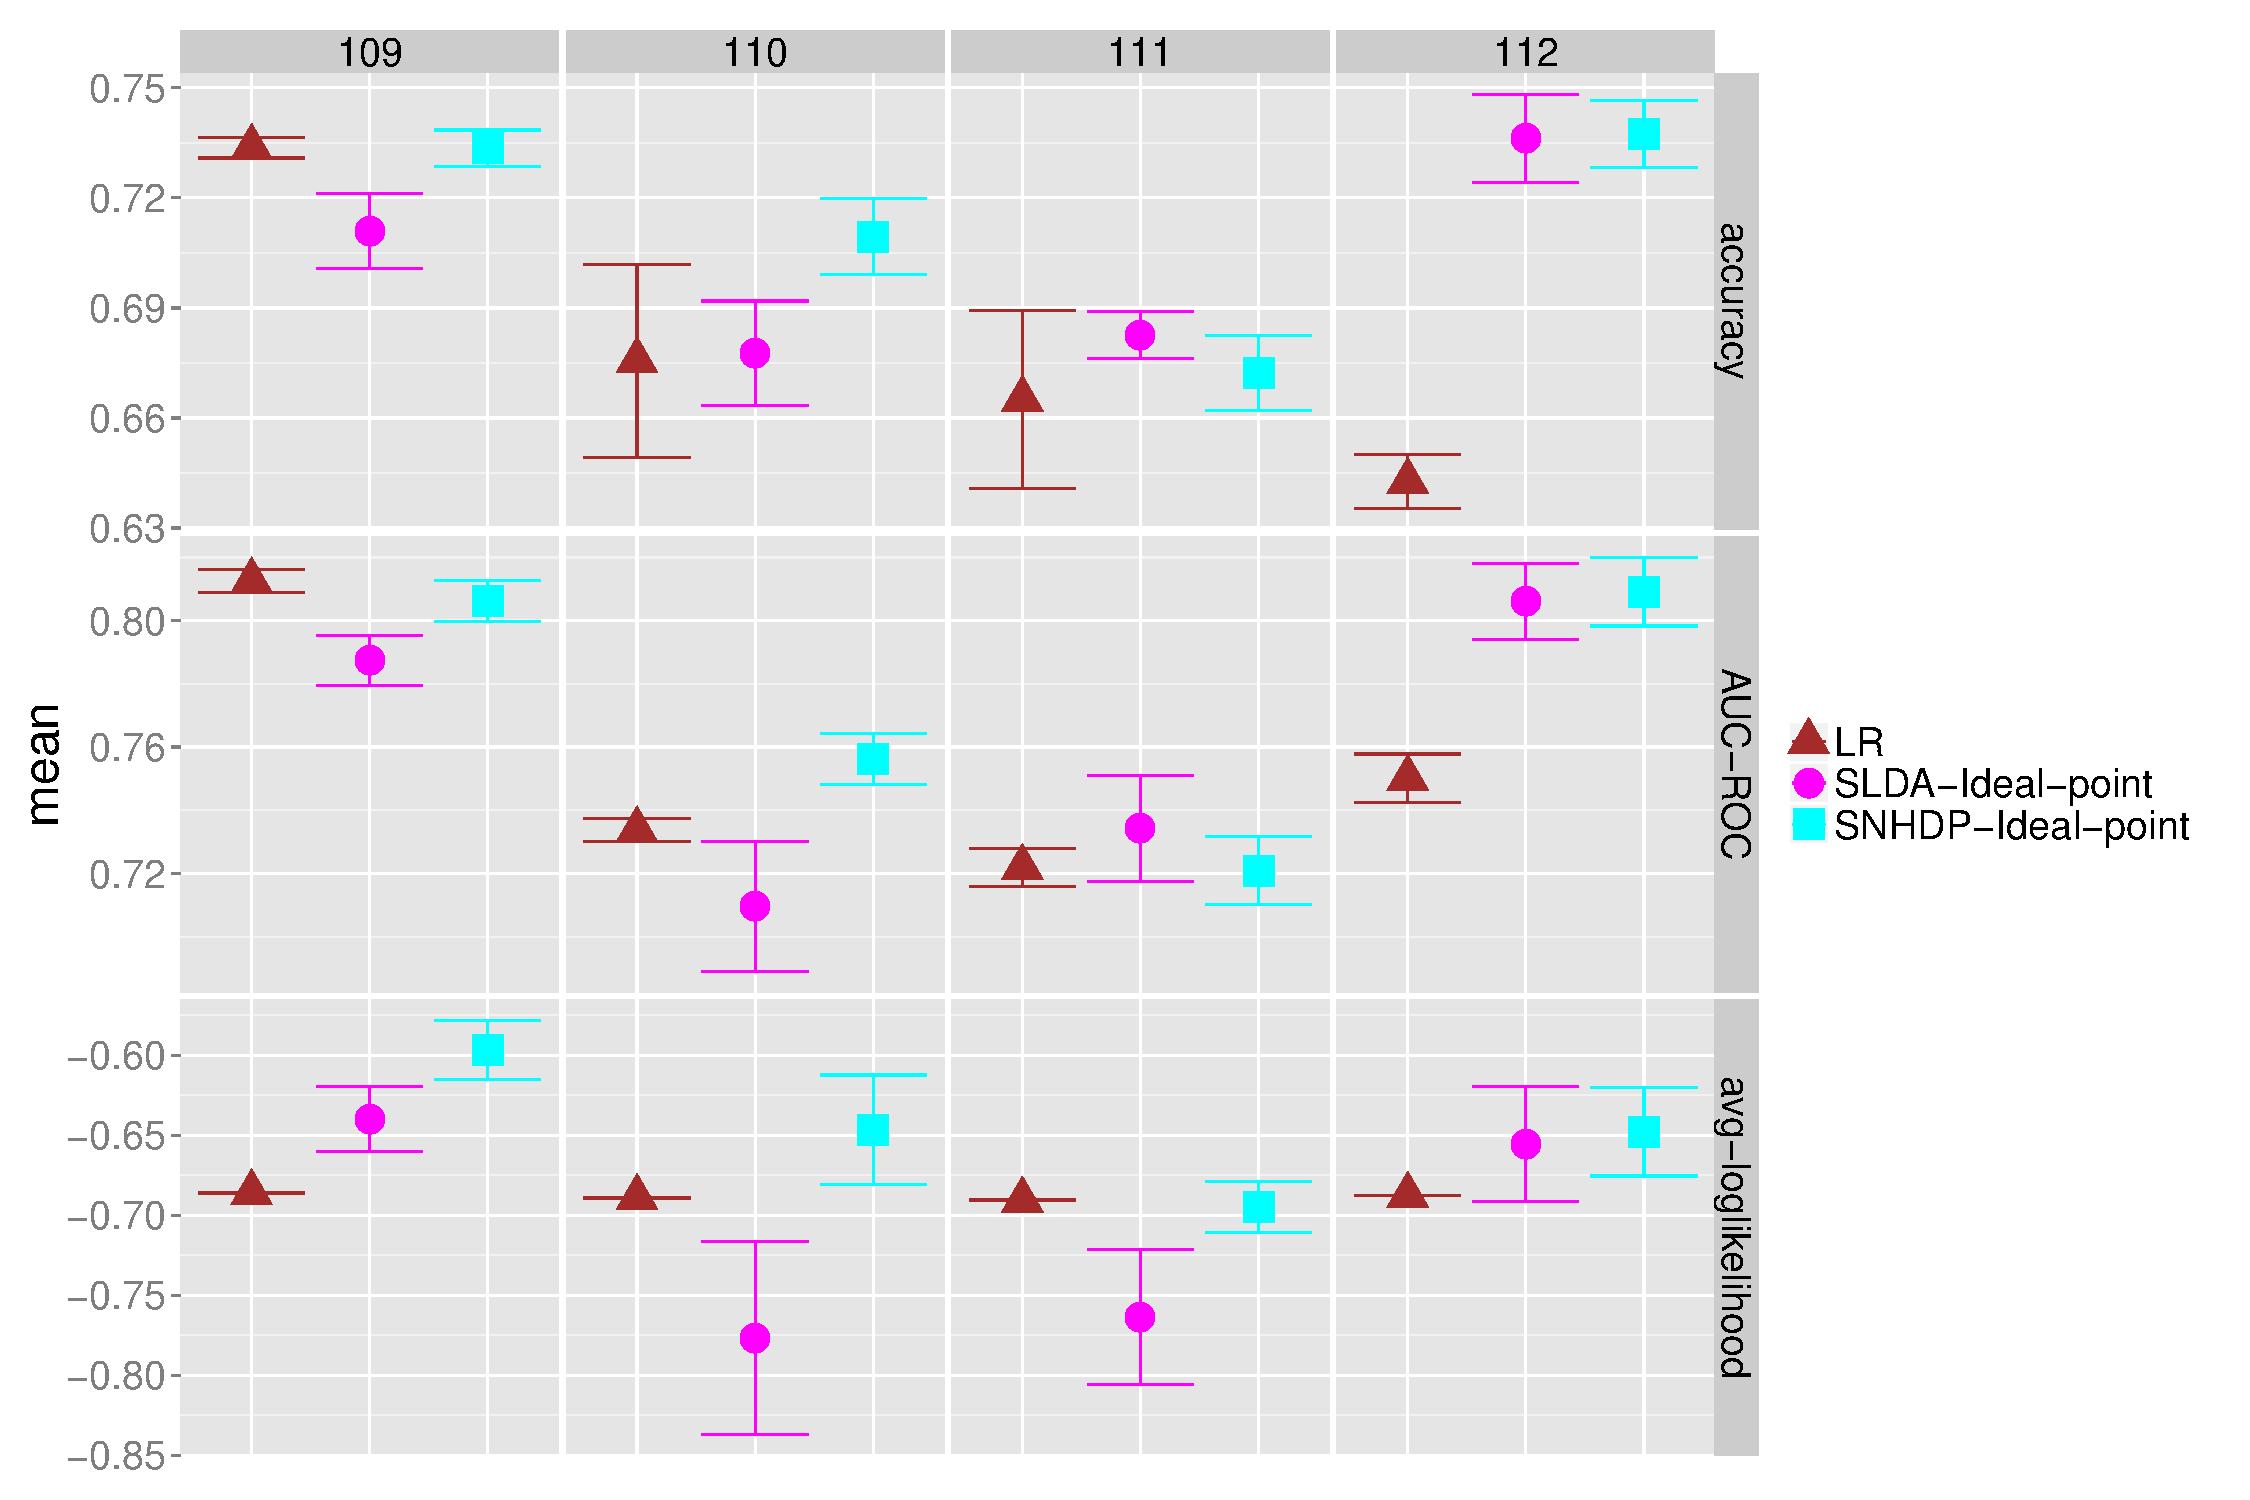
\includegraphics[width=\textwidth]{2015_teaparty/figs/heldout-authors}
%%\caption{Experiment results for predicting votes of held-out lawmakers. The results are averaged over 5 folds.}
%%\end{figure*}
%
%\subsection{Predicting held-out legislators' votes without training on bill's debates}
%\label{sec:heldout_authors debates}
%
%\begin{itemize}
%	\item word frequency
%	\item party
%	\item estimated ideal point of voters
%	\item topic distribution
%	\item score for each topic
%\end{itemize}
%
%\section{Analyzing Legislators}
%\label{sec:casestudies}
%Analyzing how Tea Partiers frame different issues on the Congressional floor.
